\iflanguage{english}
{\chapter{Appendix}}    % english style
{\chapter{Anhang}}      % german style
\label{chap:appendix}

%% ~~~~~~~~~~~~~~~~~~~~~~~~~~~~~~~~~~~~~~~~~~~~~~~~~~~~~~~~~~~~~~~~~~~~~~~ 
%%                             PyQt
%% ~~~~~~~~~~~~~~~~~~~~~~~~~~~~~~~~~~~~~~~~~~~~~~~~~~~~~~~~~~~~~~~~~~~~~~~ 

\section{PyQt}
\label{sec:appendix:pyqt}

\setcounter{figure}{0}

%% ~~~~~~~~~~~~~~~~~~~~~~~~~~~~~~~~~~~~~~~~~~~~~~~~~~~~~~~~~~~~~~~~~~~~~~~ 

\subsection{PyQt Layout Example Application Source Code}

\lstinputlisting[
    language=python,
    caption=Source code for the layout example in \ref{fig:qt:examplewindow}, 
    label=a:fig:qt:examplewindow:code
]{resources/code/windowexample.py}

\clearpage

%% ~~~~~~~~~~~~~~~~~~~~~~~~~~~~~~~~~~~~~~~~~~~~~~~~~~~~~~~~~~~~~~~~~~~~~~~ 

\subsection{Qt Event Sytem Example Application Source Code}

\lstinputlisting[
    language=python,
    caption=Source code of an example window demonstrating qts event system,
    label=a:qtevents:code
]{resources/code/event_complete.py}

\clearpage



%% ~~~~~~~~~~~~~~~~~~~~~~~~~~~~~~~~~~~~~~~~~~~~~~~~~~~~~~~~~~~~~~~~~~~~~~~ 
%%                          PyQtGraph
%% ~~~~~~~~~~~~~~~~~~~~~~~~~~~~~~~~~~~~~~~~~~~~~~~~~~~~~~~~~~~~~~~~~~~~~~~ 

\section{PyQtGraph}
\label{sec:appendix:pyqtgraph}

%% ~~~~~~~~~~~~~~~~~~~~~~~~~~~~~~~~~~~~~~~~~~~~~~~~~~~~~~~~~~~~~~~~~~~~~~~ 

\subsection{PyQtGraph PlotWidget Components Overview}

\begin{figure}[h]
    \centering
    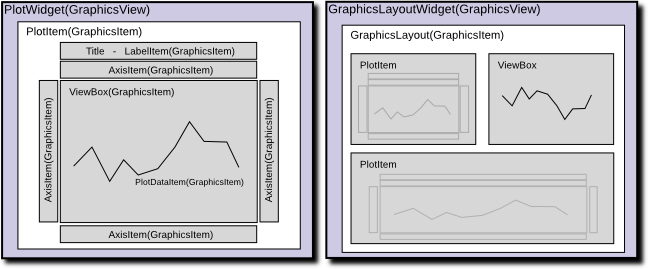
\includegraphics[width=14cm]{resources/img/PyQtGraphContent}
    \caption{Different components of a PyQtGraph plot.}
    \small\textsuperscript{Quelle: http://www.pyqtgraph.org/documentation/plotting.html}
    \label{a:fig:pyqtgraph:content}
\end{figure}

\clearpage

%% ~~~~~~~~~~~~~~~~~~~~~~~~~~~~~~~~~~~~~~~~~~~~~~~~~~~~~~~~~~~~~~~~~~~~~~~ 

\subsection{PyQtGraph PlotWidget Example Application Source Code}

\begin{figure}[h]
    \centering
    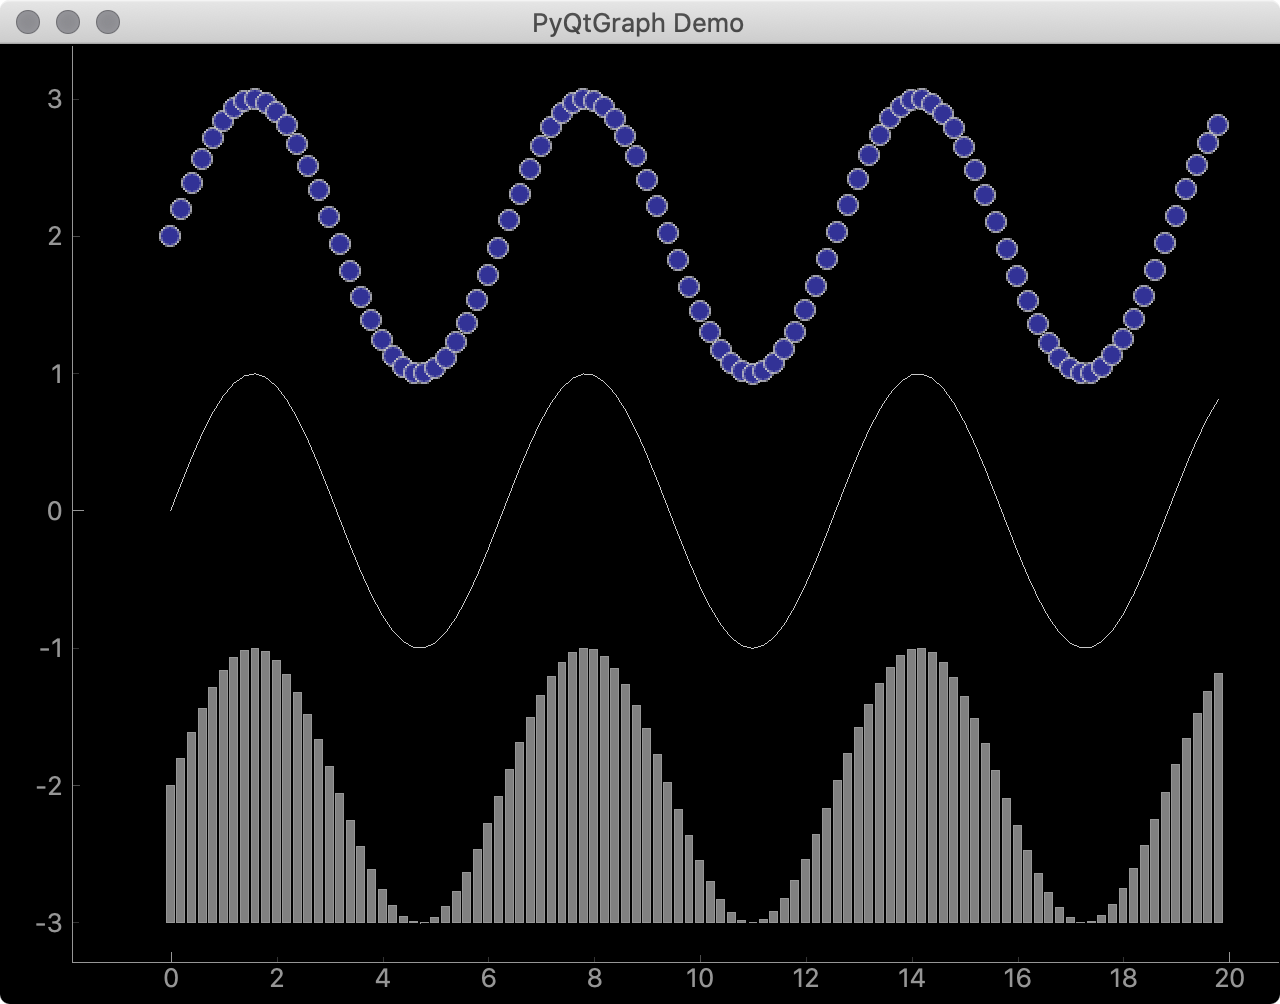
\includegraphics[width=14cm]{resources/img/PyQtGraphDemo}
    \caption{Qt Window containing a PyQtGraph plot.}
    \label{a:fig:pyqtgraph:window}
\end{figure}

\clearpage




%% ~~~~~~~~~~~~~~~~~~~~~~~~~~~~~~~~~~~~~~~~~~~~~~~~~~~~~~~~~~~~~~~~~~~~~~~ 
%%                          Matplotlib
%% ~~~~~~~~~~~~~~~~~~~~~~~~~~~~~~~~~~~~~~~~~~~~~~~~~~~~~~~~~~~~~~~~~~~~~~~ 

\section{Matplotlib}
\label{sec:appendix:matplotlib}

%% ~~~~~~~~~~~~~~~~~~~~~~~~~~~~~~~~~~~~~~~~~~~~~~~~~~~~~~~~~~~~~~~~~~~~~~~ 

\subsection{Matplotlib Figure Components Overview}

\begin{figure}[h]
    \centering
    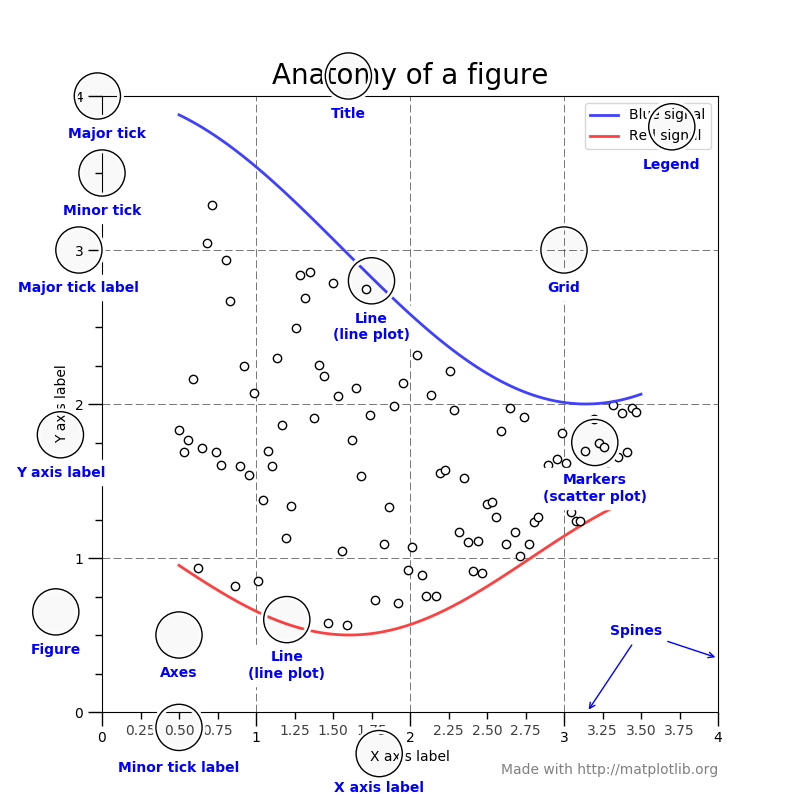
\includegraphics[width=14cm]{resources/img/MatplotlibContent}
    \caption{Different components of a Matplotlib plot.}
    \small\textsuperscript{Quelle: https://matplotlib.org/3.1.1/tutorials/introductory/usage.html}
    \label{a:fig:matplotlib:content}
\end{figure}

\clearpage

%% ~~~~~~~~~~~~~~~~~~~~~~~~~~~~~~~~~~~~~~~~~~~~~~~~~~~~~~~~~~~~~~~~~~~~~~~ 

\subsection{Matplotlib Figure Example Application Source Code}

\begin{figure}[h]
    \centering
    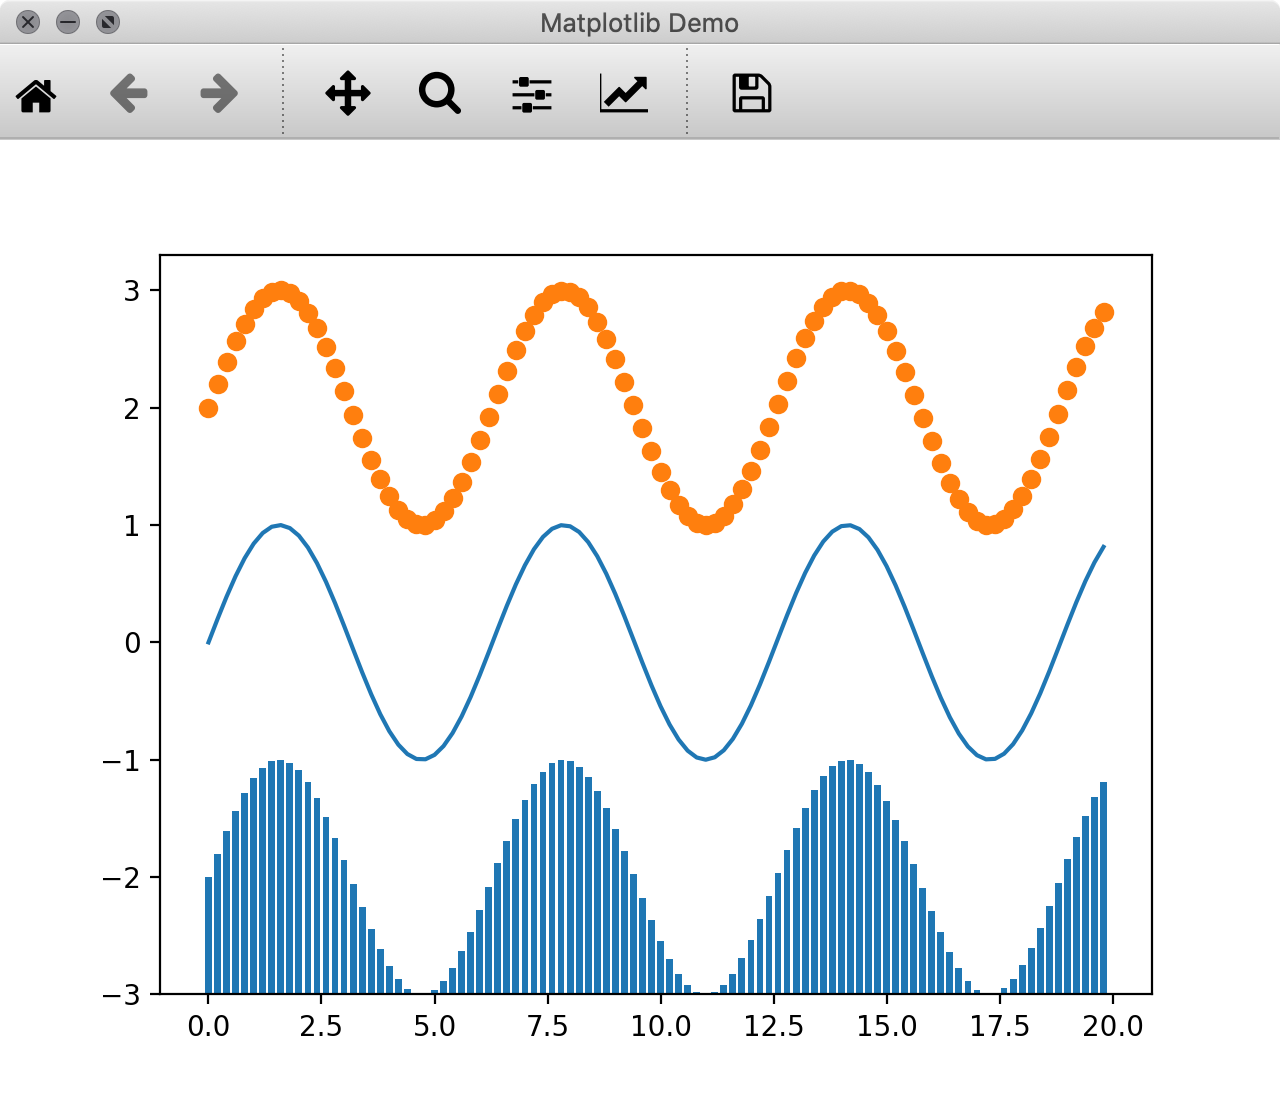
\includegraphics[width=14cm]{resources/img/MatplotlibDemo}
    \caption{Qt Window containing a Matplotlib plot.}
    \label{a:fig:matplotlib:window}
\end{figure}

\clearpage




%% ~~~~~~~~~~~~~~~~~~~~~~~~~~~~~~~~~~~~~~~~~~~~~~~~~~~~~~~~~~~~~~~~~~~~~~~ 
%%                          Evaluation
%% ~~~~~~~~~~~~~~~~~~~~~~~~~~~~~~~~~~~~~~~~~~~~~~~~~~~~~~~~~~~~~~~~~~~~~~~ 

\section{Evaluation}
\label{sec:appendix:evaluation}

%% ~~~~~~~~~~~~~~~~~~~~~~~~~~~~~~~~~~~~~~~~~~~~~~~~~~~~~~~~~~~~~~~~~~~~~~~ 

\subsection{Delta Times for 1,000 Points}

\begin{figure}[h]
    \centering
    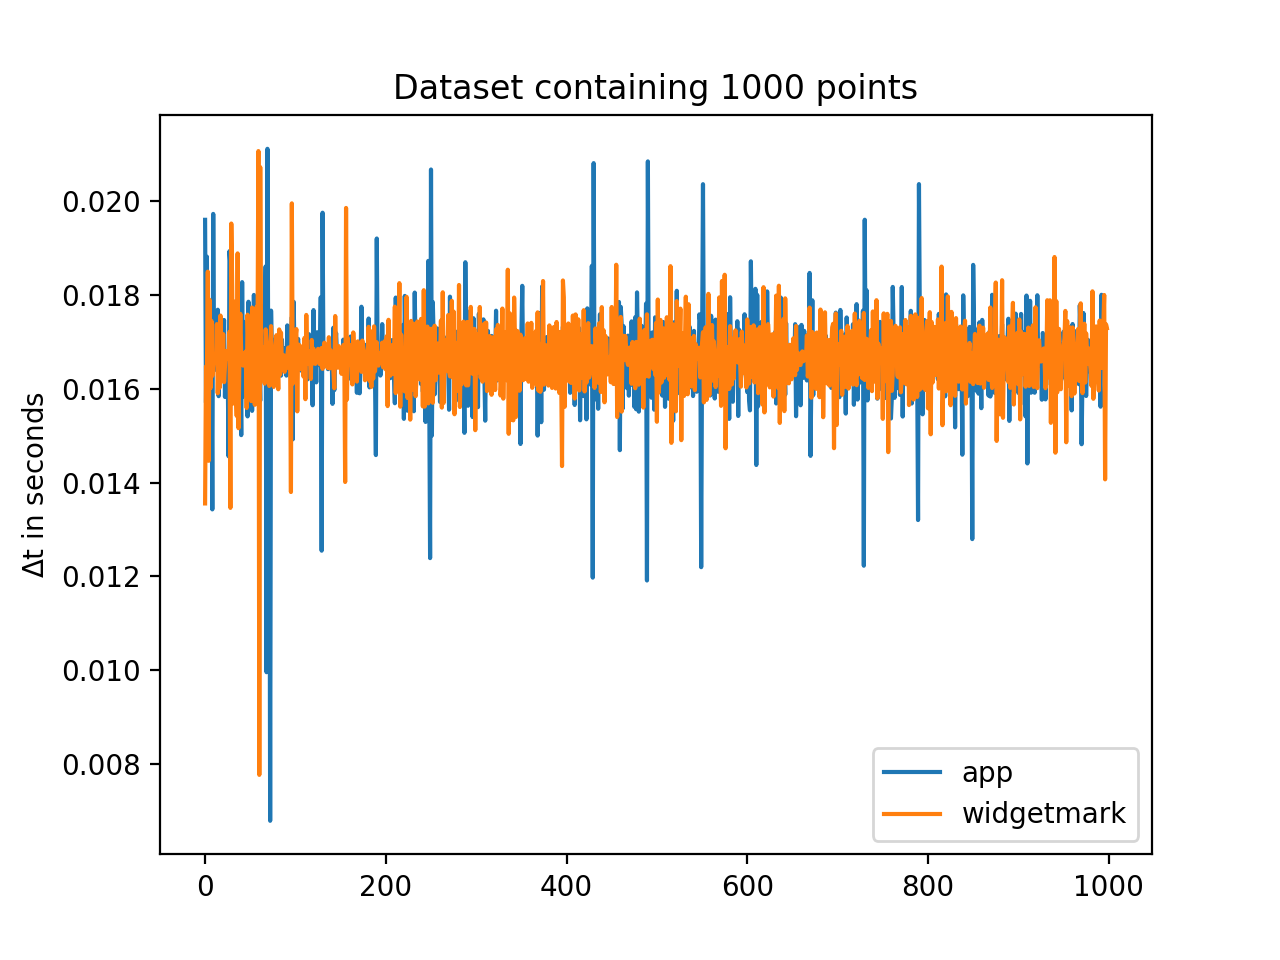
\includegraphics[width=14cm]{resources/img/evaluation/Eval_1000}
    \caption{
        Recorded Delta Times for a 1,000 point data set
    }
    \label{a:tab:evaluation:1000}
\end{figure}

\clearpage

%% ~~~~~~~~~~~~~~~~~~~~~~~~~~~~~~~~~~~~~~~~~~~~~~~~~~~~~~~~~~~~~~~~~~~~~~~ 

\subsection{Delta Times for 10,000 Points}

\begin{figure}[h]
    \centering
    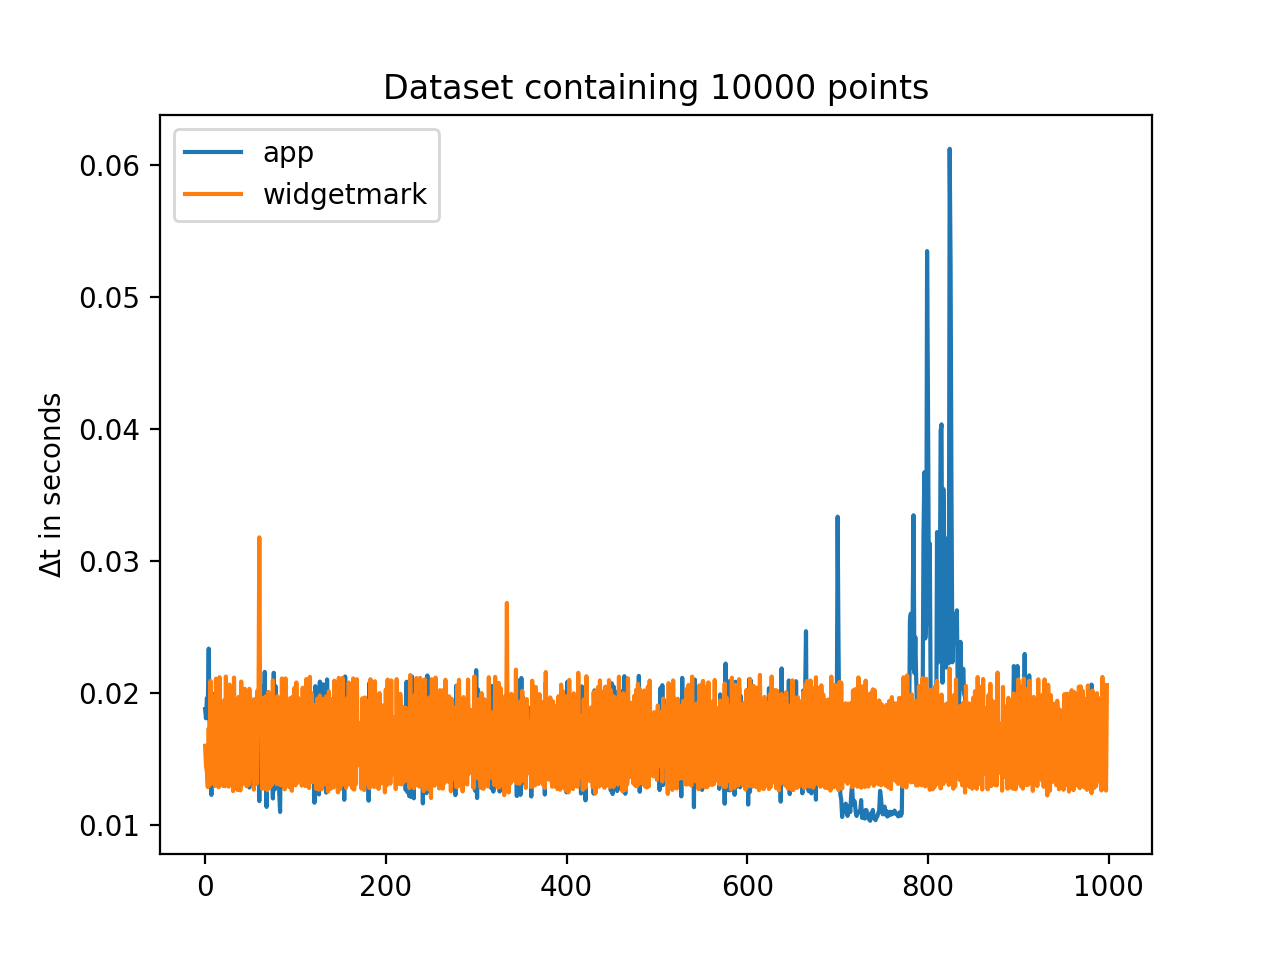
\includegraphics[width=14cm]{resources/img/evaluation/Eval_10000}
    \caption{
        Recorded Delta Times for a 10,000 point data set
    }
    \label{a:tab:evaluation:10000}
\end{figure}

\clearpage

%% ~~~~~~~~~~~~~~~~~~~~~~~~~~~~~~~~~~~~~~~~~~~~~~~~~~~~~~~~~~~~~~~~~~~~~~~ 

\subsection{Delta Times for 50,000 Points}

\begin{figure}[h]
    \centering
    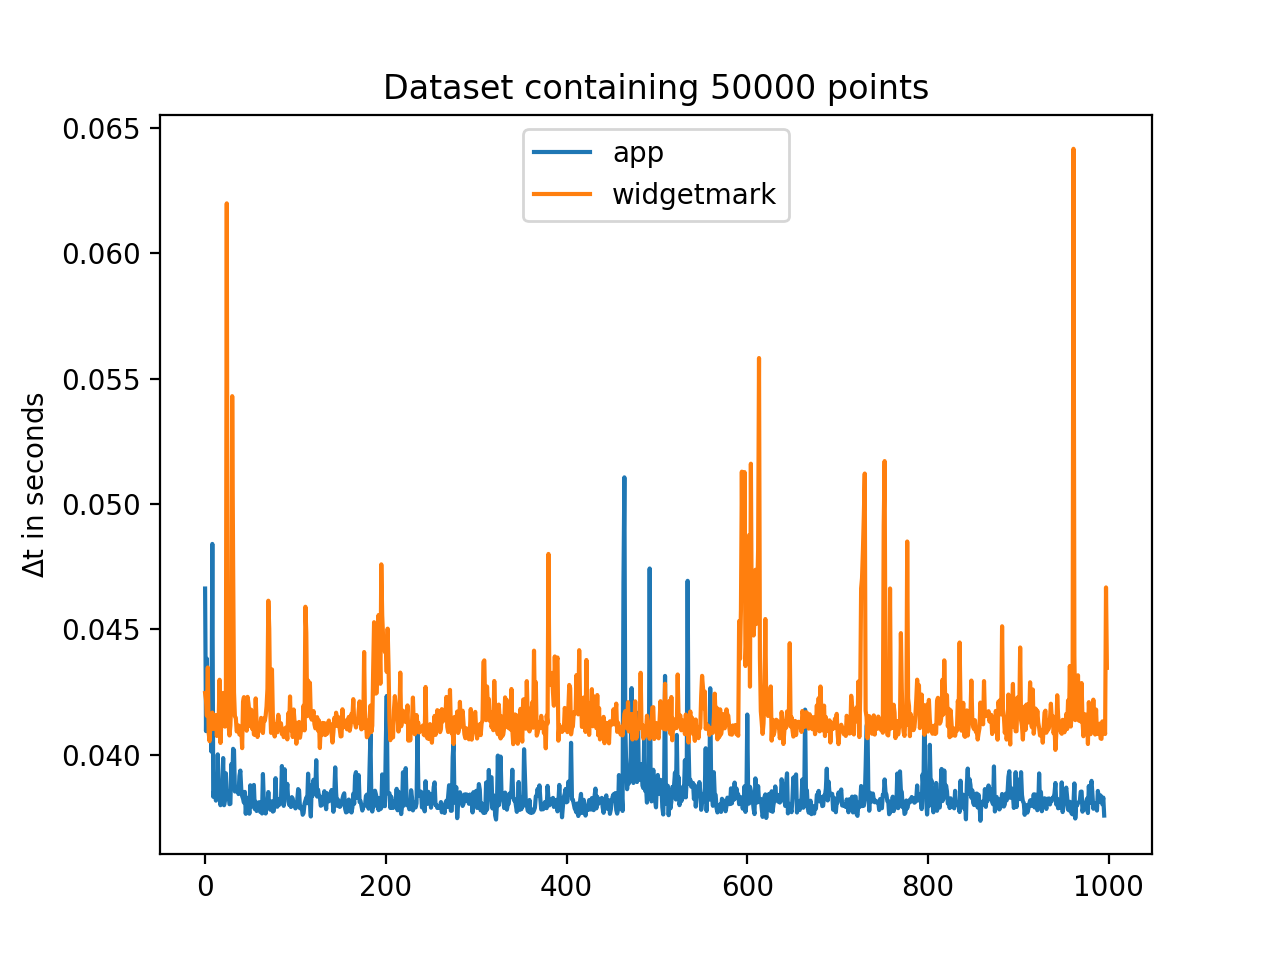
\includegraphics[width=14cm]{resources/img/evaluation/Eval_50000}
    \caption{
        Recorded Delta Times for a 50,000 point data set
    }
    \label{a:tab:evaluation:50000}
\end{figure}

\clearpage

%% ~~~~~~~~~~~~~~~~~~~~~~~~~~~~~~~~~~~~~~~~~~~~~~~~~~~~~~~~~~~~~~~~~~~~~~~ 

\subsection{Delta Times for 100,000 Points}

\begin{figure}[h]
    \centering
    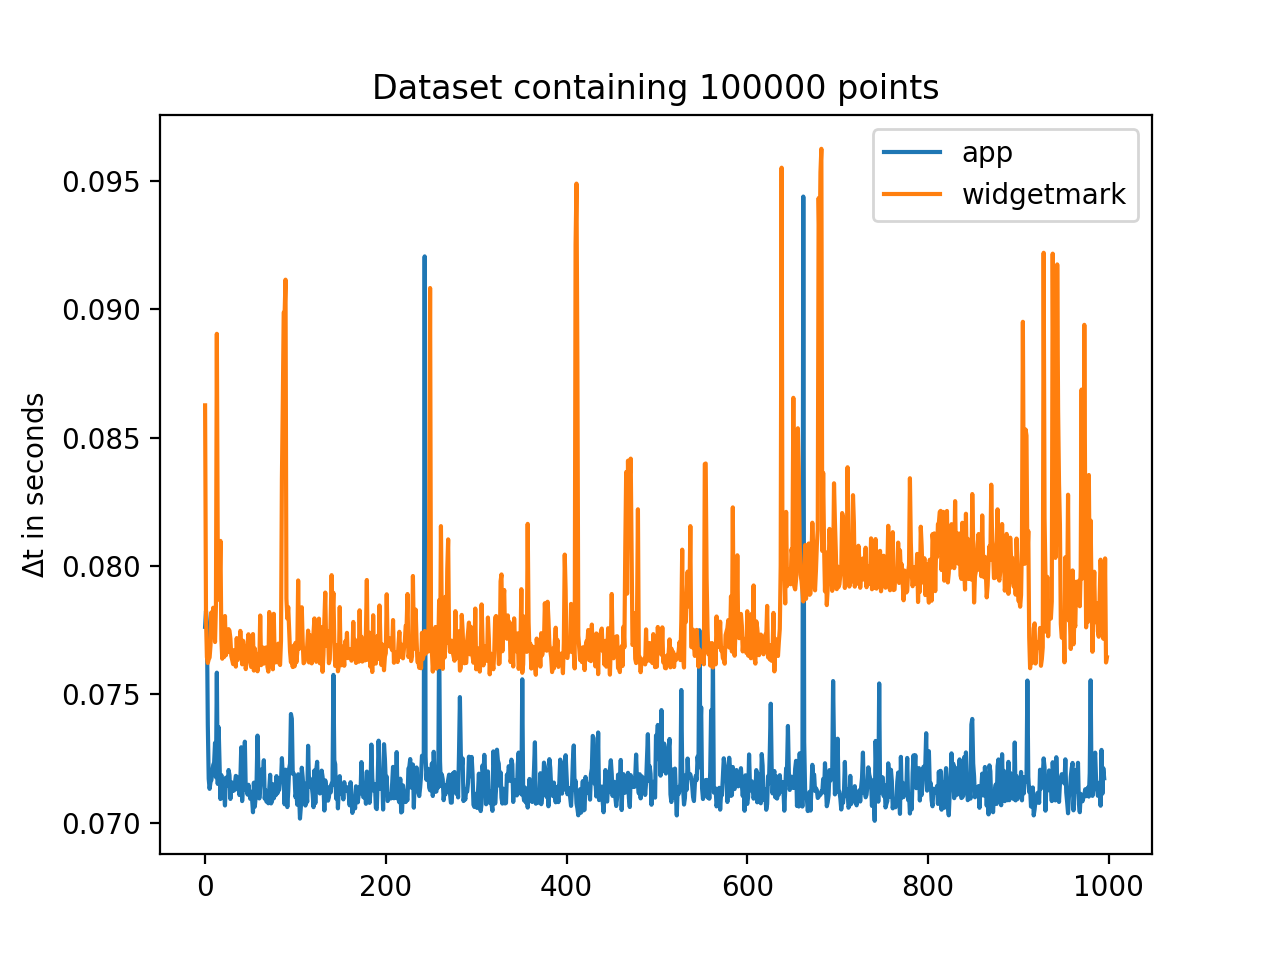
\includegraphics[width=14cm]{resources/img/evaluation/Eval_100000}
    \caption{
        Recorded Delta Times for a 100,000 point data set
    }
    \label{a:tab:evaluation:100000}
\end{figure}

\clearpage

%% ~~~~~~~~~~~~~~~~~~~~~~~~~~~~~~~~~~~~~~~~~~~~~~~~~~~~~~~~~~~~~~~~~~~~~~~ 

\subsection{PyQt Comparison Application Source Code}

\lstinputlisting[
    caption=PyQt comparison application used in the evaluation of the framework's accuracy,
    language=python, 
    label=listing:evaluation:pyqtapp
]{resources/widgetmark/evaluation/app.py}

\clearpage

%% ~~~~~~~~~~~~~~~~~~~~~~~~~~~~~~~~~~~~~~~~~~~~~~~~~~~~~~~~~~~~~~~~~~~~~~~ 

\subsection{Evaluation Use Case Source Code}

\lstinputlisting[
    caption=Evaluation use case used in the evaluation of the framework's accuracy,
    language=python, 
    label=listing:evaluation:usecase
]{resources/widgetmark/evaluation/usecase.py}
